\section{Methods}
\label{sec:methods}

In this manuscript, we are primarily concerned with $k$-NN search in a finite-dimensional space.
Given a dataset $\textbf{X} = \{x_1 \dots x_n\}$ of cardinality $|\textbf{X}| = n$, we define a \textit{point} or \textit{datum} $x_i \in \textbf{X}$ as a singular observation. Examples include the neural-network embedding of an image, the genome of an organism, and a measurement of a radio frequency signal.

We define a \textit{distance function} $f : \textbf{X} \times \textbf{X} \mapsto \mathbb{R}^+ \ \cup \ \{0\}$ which, given two points, deterministically returns a finite and non-negative real number.
A distance value of zero defines an identity among points (i.e. $f(x, y) = 0 \Leftrightarrow x = y$) and larger values indicate greater dissimilarity among the points.
We also require that the distance function be symmetric (i.e., $f(x, y) = f(y, x) \ \forall \ x, y \in \textbf{X}$).
In addition to these constraints, if the distance function obeys the triangle inequality (i.e. $f(x, y) \leq f(x, z) + f(z, y) \ \forall \ x, y, z \in \textbf{X}$), then it is also a \textit{distance metric}.
Similar to~\cite{yu2015entropy}, when used with distance metrics, all search algorithms in CAKES are exact.
For example, Euclidean, Levenshtein~\cite{levenshtein1966binary} and Dynamic Time Warping (DTW)~\cite{muller2007dynamic} distances are all distance metrics, while Cosine distance is not a metric because it violates the triangle inequality (e.g., consider the points $x = (1, 0)$, $y = (0, 1)$ and $z = (1, 1)$ on the Cartesian plane).

The choice of an appropriate distance function varies by dataset and domain.
For example, with neural-network embeddings, one could use Euclidean (L2) or Cosine distance.
With genomic or proteomic data, Levenshtein, Smith-Waterman, Needleman-Wunsch or Hamming distances are useful.
With time-series data, one could use Dynamic Time Warping (DTW) or Wasserstein distance.

CAKES assumes the manifold hypothesis~\cite{fefferman2016testing}, the notion that high-dimensional data collected from constrained generating phenomena typically only occupy a low-dimensional manifold within their embedding space.
We say that such data are \textit{manifold-constrained} and have low \textit{local fractal dimension} (LFD).
In other words, we assume that the dataset is embedded in a $D$-dimensional space, but that the data only occupy a $d$-dimensional manifold, where $d \ll D$.
While we sometimes use Euclidean notions, such as voids, volumes and proximity to describe the geometric and topological properties of the clusters and manifold, CLAM and CAKES do not rely on such notions;
they serve merely as convenient and intuitive vocabulary to discuss the underlying mathematics.

CAKES exploits the low LFD of such datasets to accelerate search.
We define LFD at some length scale around a point in the dataset as:

\begin{equation}
    \frac{\text{log} \left( \frac{|B_X(q, r_1)|}{|B_X(q, r_2)|} \right) }{\text{log} \left( \frac{r_1}{r_2} \right) }
    \label{eq:methods:lfd-original}
\end{equation}
where $B_X(q, r)$ is the set of points contained in the metric ball of radius $r$ centered at a point $q$ in the dataset $\textbf{X}$.
Intuitively, LFD measures the rate of change in the number of points in a ball of radius $r$ around a point $q$ as $r$ increases. When the vast majority of points in the dataset have low ($\ll D$) LFD, we can overload terminology to say that the dataset has low LFD.

We stress that this concept differs from the \textit{embedding dimension} of a dataset.
To illustrate the difference, consider the SILVA 18S rRNA dataset which contains genomes with unaligned lengths of up to 3,718 base pairs and aligned length of 50,000 base pairs.
Hence, the \textit{embedding dimension} of this dataset is at least 3,718 and at most 50,000.
However, due to physical constraints (namely, biological evolution and the chemistry of RNA replication and mutation processes), the data are constrained to a lower-dimensional manifold within this embedding space.
LFD is an approximation of the dimensionality of that lower-dimensional manifold in the ``vicinity'' of a given point.
Figure~\ref{fig:results:lfd-plots} illustrates this concept on a variety of datasets, showing how real datasets uphold the manifold hypothesis.


\subsection{Clustering}
\label{sec:methods:clustering}

We define a \textit{cluster} as a set of points with a \textit{center} and a \textit{radius}.
The \textit{center} is the geometric median of the points (or a smaller sample of the points) in the \textit{cluster}, and so it is a real data point.
The \textit{radius} is the maximum distance from the \textit{center} to any point in the \textit{cluster}.
Each non-leaf cluster has two child clusters in much the same way that a node in a binary tree has two child nodes.
Note that clusters can have overlapping volumes and, in such cases, points in the overlapping volume are assigned to exactly one of the overlapping clusters.
As a consequence, a cluster can be a proper subset of the metric ball at the same center and radius, i.e. $C(c, r) \subset B_X(c, r)$.

Hereafter, when we refer to the LFD of a \textit{cluster}, it is estimated at the length scale of the cluster radius and half that radius.
This allows us to rewrite Definition~\ref{eq:methods:lfd-original} as:

\begin{equation}
    \log_2 \left( \frac{|C(c, r)|}{|C(c, \frac{r}{2})|} \right)
    \label{eq:methods:lfd-simplified}
\end{equation}

where $|C(c, r)|$ is the cardinality of the cluster $C$ with center $c$ and radius $r$, and $C(c, \frac{r}{2})$ is the set of points in $C$ which are no more than a distance $\frac{r}{2}$ from $c$, i.e. $C(c, \frac{r}{2}) = \{p : p \in C \land f(c, p) \leq \frac{r}{2}\}$.

The \textit{metric entropy} $\mathcal{N}_{r}(X)$ for some radius $r$ was defined, in~\cite{yu2015entropy}, as the minimum number of clusters of a uniform radius $r$ needed to cover the data.
In this paper, where the clustering is hierarchical rather than flat, we define the metric entropy $\mathcal{N}_{\hat{r}}(X)$ of a dataset $X$ as the number of leaf clusters in the tree where $\hat{r}$ is the mean radius of all leaf clusters.

We start by performing a divisive hierarchical clustering on the dataset using CLAM.
The procedure is similar to that outlined in CHESS, but with the following improvements:
better selection of poles for partitioning (see Algorithm~\ref{alg:methods:partition}) and depth-first reordering of the dataset (see Section~\ref{sec:methods:clustering:depth-first-reordering}).


\subsubsection{Building the Tree}
\label{sec:methods:clustering:building-the-tree}

CLAM starts by building a binary tree of clusters using a divisive hierarchical clustering algorithm.

For a cluster $C$ with $|C|$ points, we begin by taking a random sample of $\sqrt{|C|}$ of its points, and computing pairwise distances between all points in this sample.
Using these distances, we compute the \textit{geometric median} of this sample; in other words, we find the point which minimizes the sum of distances to all other points in the sample.
This geometric median is the \textit{center} of $C$.

The \textit{radius} of $C$ is the maximum distance from the \textit{center} to any other point in $C$.
The point which is responsible for that radius (i.e., the furthest point from the center) is designated the \textit{left pole} and the point which is furthest from the left pole is designated the \textit{right pole}.

We then partition the cluster into a \textit{left child} and a \textit{right child}, where the left child contains all points in the cluster which are closer to the left pole than to the right pole, and the right child contains all points in the cluster which are closer to the right pole than to the left pole.
Without loss of generality, we assign to the left child those points which are equidistant from the two poles.

Starting from a root cluster containing the entire dataset, we repeat this procedure until each leaf contains only one datum, or we meet some other user-specified stopping criteria, for example, minimum cluster radius, minimum cluster cardinality, maximum tree depth, etc.
This process is described in Algorithm \ref{alg:methods:partition}.

During the partitioning process, we also compute (and cache) the LFD of each cluster using Equation~\ref{eq:methods:lfd-simplified}.

\begin{algorithm} % enter the algorithm environment
    \caption{Partition($C$, $criteria$)} % give the algorithm a caption
    \label{alg:methods:partition} % and a label for \ref{} commands later in the document
    \begin{algorithmic}[0] % enter the algorithmic environment
        \Require $C$, a cluster
        \Require $criteria$, user-specified stopping criteria

        \State $seeds \Leftarrow$ random sample of $\left\lceil \sqrt{|C|} \right\rceil$ points from $C$
        \State $c \Leftarrow$ geometric median of $seeds$
        \State $l \Leftarrow \argmax f(c, x) \ \forall \ x \in C$
        \State $r \Leftarrow \argmax f(l, x) \ \forall \ x \in C$
        \State $L \Leftarrow \{x \ | \ x \in C \land f(l, x) \le f(r, x)\}$
        \State $R \Leftarrow \{x \ | \ x \in C \land f(r, x) < f(l, x)\}$
        
        \If{$|L| > 1$ \textbf{and} $L$ satisfies $criteria$}
            \State Partition($L$, $criteria$)
        \EndIf
        
        \If{$|R| > 1$ \textbf{and} $R$ satisfies $criteria$}
            \State Partition($R$, $criteria$)
        \EndIf
    \end{algorithmic}
\end{algorithm}

Note that Algorithm~\ref{alg:methods:partition} does not necessarily produce a balanced tree.
In fact, for real datasets, we expect anything but a balanced tree; the varying sampling density in different regions of the manifold and the low dimensional ``shape'' of the manifold itself will cause it to be unbalanced.
The only case in which we would expect a balanced tree is if the dataset were uniformly distributed, e.g. in a $d$-dimensional hyper-cube.
In this sense, the imbalance in the tree is a feature, not a bug, as it reflects the underlying structure of the data.


\subsubsection{Depth-First Reordering}
\label{sec:methods:clustering:depth-first-reordering}

After building the tree, we reorder the dataset so that the points are stored in the order that they would be visited during a depth-first traversal of the tree.

In CHESS, each cluster stored a list of indices into the dataset.
This list was used to retrieve the clusters' points during search.
Although this approach allowed us to retrieve the points in constant time, its memory cost was prohibitively high.
With a dataset of cardinality $n$ and each cluster storing a list of indices for its points, we stored a total of $n$ indices at each depth in the tree.
Assuming a balanced tree, and thus $\mathcal{O}(\log n)$ depth, this approach had a memory overhead of $\mathcal{O}(n \log n)$.

One may improve this memory overhead to $\mathcal{O}(n)$ by only storing indices at the leaf clusters.
This approach, however, introduces a time cost of $\mathcal{O}(n \log n)$ whenever we need to find the indices for a non-leaf cluster (because it requires a traversal of the subtree rooted at that cluster).

In this work, we introduce a new approach wherein, after building the cluster tree, we reorder the dataset so that points are stored in a depth-first order.
Then, within each cluster, we need only store its \textit{cardinality} and an \textit{offset} to access its points from the dataset.
The root cluster has an offset of zero and a cardinality equal to the number of points in the dataset.
A left child has the same offset as that of its parent, and the corresponding right child has an offset equal to the left child's offset plus the left child's cardinality.

With no additional memory cost nor time cost for retrieving points during search, depth-first reordering offers significant improvements at search-time over the approach used in CHESS.

% % WE WILL USE THIS FOR COMPRESSION. DO NOT DELETE

% \subsubsection{Scaling Behavior of Cluster Radii}
% \label{sec:methods:clustering:scaling-behabior-of-cluster-radii}

% While it may be tempting to assume that cluster radii decrease with each application of Partition (refer to Algorithm \ref{alg:methods:partition}), unfortunately, this assumption is incorrect. 
% Fortunately, we \textit{can} make some guarantees about the scaling behavior of cluster radii;
% in particular, we prove in this section that cluster radii will stop increasing after at most $d$ partitions, where $d$ is the fractal dimensionality of the dataset. 

% We can describe a $d$-dimensional distribution of data by choosing some set of $d$ mutually orthogonal axes.
% Let $2R$ be the maximum pairwise distance among the points in the dataset. 
% We choose the axes such that the two points that are $2R$ apart lie \textit{along one of the axes}. 
% Thus, a $d$-dimensional hyper-sphere of radius $R$ would bound the dataset. 
% In the worst case, (i.e., with a uniform-density distribution that fills the $d$-sphere), our axes will be such that $2R$ is the maximum pairwise distance \textit{along every axis}. 
% Such a distribution would also produce a balanced cluster tree.

% In this case, Partition will select a maximally distant pair of points to use as poles;
% without loss of generality, say it chooses two points at the extrema one of the $d$ axes. 
% After one partition, the maximum pairwise distance along that axis will be halved, i.e. bounded above by $R$.
% The next recursive Partition will select another of the $d$ axes, and once again, the distance along that axis will be bounded above by $R$
% Thus, after at most $d$ partitions, the maximum pairwise distance along each axis will be bounded above by $R$. 
% The overall (i.e., not restricted to one axis) maximum pairwise distance 
% will be bounded above by $R\sqrt{2}$ by, for example, two instances that lie at the extrema of different axes. 
% See Figure~\ref{fig:methods:radii-scaling-behavior} for an example.

% Thus, starting with a cluster $C$ of radius $R$, after at most $d$ Partitions, the descendants of $C$ will each have radius
% bounded above by $\frac{R}{\sqrt{2}}$. In other words, cluster radii are guaranteed to decrease by a multiplicative factor of $\frac{\sqrt{2}}{2}$ after at 
% most $d$ partitions. 

% Note that, in practice, we never see a balanced clustering.
% Partition produces unbalanced trees due to the varying density of the sampling in different regions of the manifold and the low dimensional ``shape'' of the manifold.
% Further, in practice, the cluster radii decrease by a factor much larger than $\frac{\sqrt{2}}{2}$ with almost every partition;
% the upper bound of $d$ partitions is seldom realized. 

% \begin{figure}[ht!]
%     \centering
%     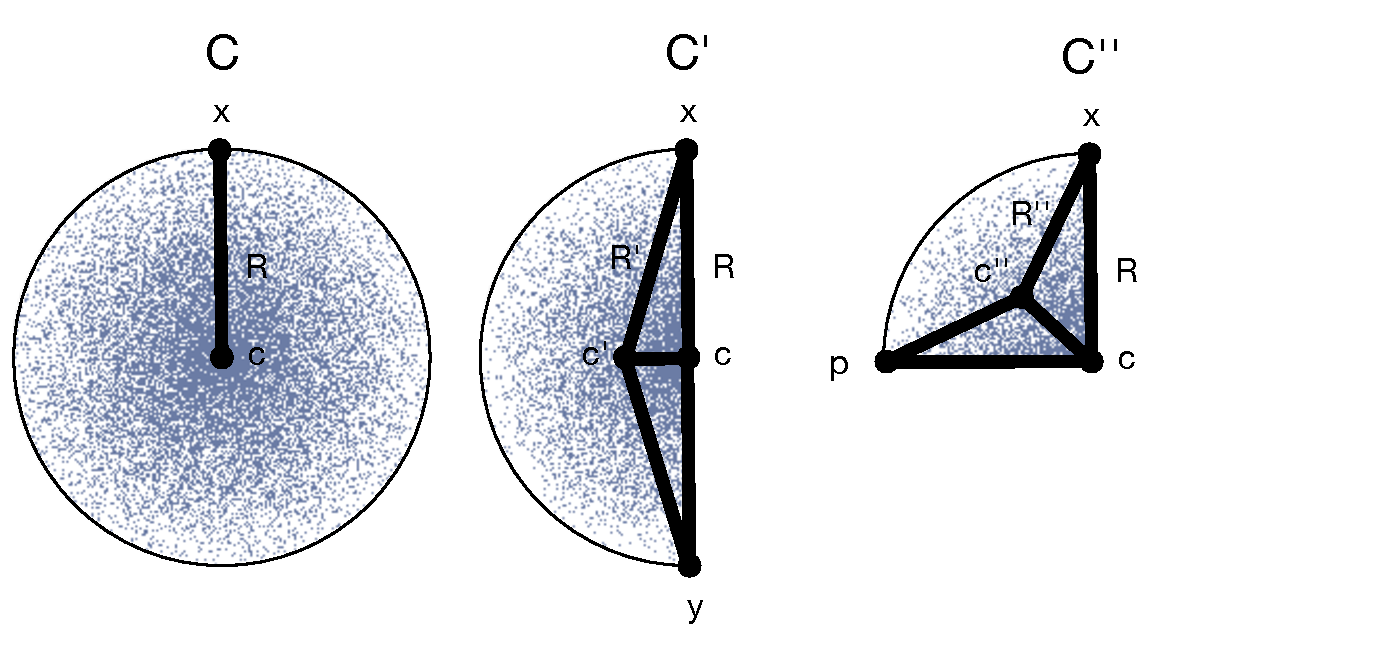
\includegraphics[width=3.4in]{images/geometry/geometry.pdf}
%     \caption{
%         Scaling behavior of radii on a uniform-density disk, which represents the worst-case scenario for a two-dimensional distribution. 
%         $R_0$ denotes the radius of the root cluster $C_0$, and $o_0$ denotes its center. 
%         After one application of Algorithm~\ref{alg:methods:clustering:partition}, we have $C_1$, with radius $R_1$ and center $o_1$.
%         The right triangle formed by $o_0$, $o_1$, and $y_+$ in $C_1$ shows that $R_0 < R_1$.
%         Hence, the radius of a child cluster can be larger than its parent.
%         However, after another application of Algorithm~\ref{alg:methods:clustering:partition}, we have consumed all $d$ orthogonal axes, 
%         as shown in $C_2$.
%         Now, clearly $R_2 < R_0$.
%         In fact, for each subsequent application of Algorithm~\ref{alg:methods:clustering:partition}, the radius of the resulting cluster is bounded above by $\frac{\sqrt{2}R}{2}$.
%     }
%     \label{fig:methods:radii-scaling-behavior}
% \end{figure}


\subsubsection{Complexity}
\label{sec:methods:clustering:complexity}

The asymptotic complexity of Partition is the same as described in~\cite{ishaq2019clustered}.
By using an approximate partitioning with a $\sqrt{n}$ sample, we achieve $\mathcal{O}(n)$ cost of partitioning and $\mathcal{O}(n \log n)$ cost of building the tree.
This is a significant improvement over exact partitioning and tree-building, which cost $\mathcal{O}(n^2)$ and $\mathcal{O}(n^2 \log n)$ respectively.


\subsection{The Search Problem}
\label{sec:methods:the-search-problem}

Given Algorithm~\ref{alg:methods:partition}, we can now formally pose the $k$-NN and $\rho$-NN search problems.

Given a query $q$, along with a distance function $f$ defined on a dataset $\textbf{X}$, we define the $k$-NN search problem, which aims to find the $k$ closest points to $q$ in $\textbf{X}$;
in other words, $k$-NN search aims to find the set $H$ such that $|H| = k$ and $H = B_X(q, \rho_k)$ where $\rho_k = \max \left\{ f(q, p) \ \forall \ p \in H \right\}$ is the distance from $q$ to the $k^{th}$ nearest neighbor in $\textbf{X}$.
We also have the $\rho$-NN search problem, which aims to find the all points in $\textbf{X}$ that are no more than a distance $\rho$ from $q$: the set $H = B_X(q, \rho) = \{x \in \textbf{X}: f(q, x) \leq \rho \}$.

Given a cluster $C$, let $c$ be its center and $r$ be its radius.
Our $\rho$-NN and $k$-NN search algorithms make use of the following properties, as illustrated in Figure~\ref{fig:methods:deltas}.

\begin{itemize}
    \item $\delta = f(q, c)$, the distance from the query to the cluster center $c$.
    \item $\delta^{+} = \delta + r$, the distance from the query to the theoretically farthest point in $C$.
    \item $\delta^{-} = \text{max}(0, \delta - r)$, the distance from the query to the theoretically closest point in $C$.
\end{itemize}

\begin{figure}[ht!]
    \centering
    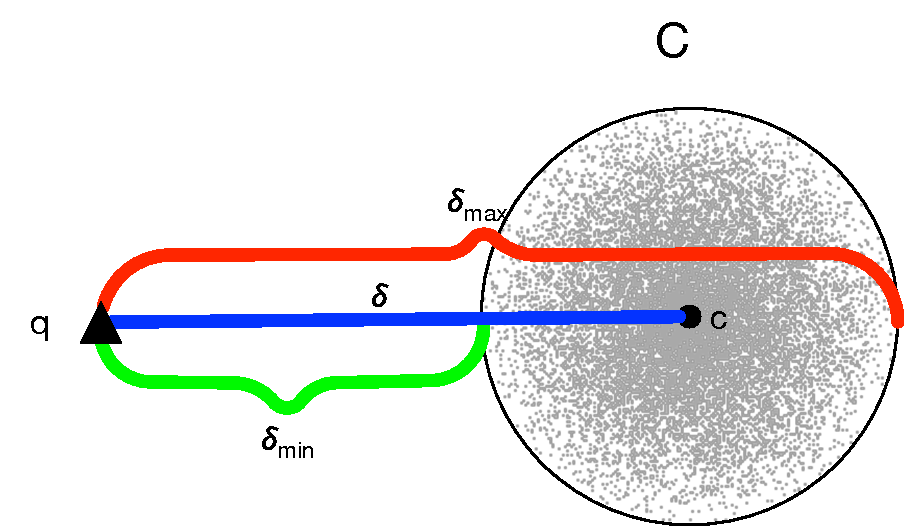
\includegraphics[scale=0.8]{images/geometry/deltas.pdf}
    \caption{{\color{blue}$\delta$}, {\color{red}$\delta^{+}$}, and {\color{green}$\delta^{-}$} for a cluster $C$ and a query $q$.}
    \label{fig:methods:deltas}
\end{figure}

We define a \textit{singleton} as a cluster which either contains a single point (i.e., has cardinality 1) or which contains only duplicates of the same point (i.e., has cardinality greater than 1 but contains only one \textit{unique} point).
A singleton clearly has zero radius, and so $\delta = \delta^{-} = \delta^{+}$.
Hence, we overload the above notation to also refer to the distance from a query to an individual point.


\subsection{\texorpdfstring{$\rho$}{p}-Nearest Neighbors Search}
\label{sec:methods:rnn-search}

We conduct $\rho$-NN search as described in~\cite{ishaq2019clustered}, but with the following improvement:
when a cluster overlaps with the query ball, instead of always proceeding to search both of its children, we proceed only with those children which might contain points in the query ball.

\begin{figure}[ht!]
    \centering
    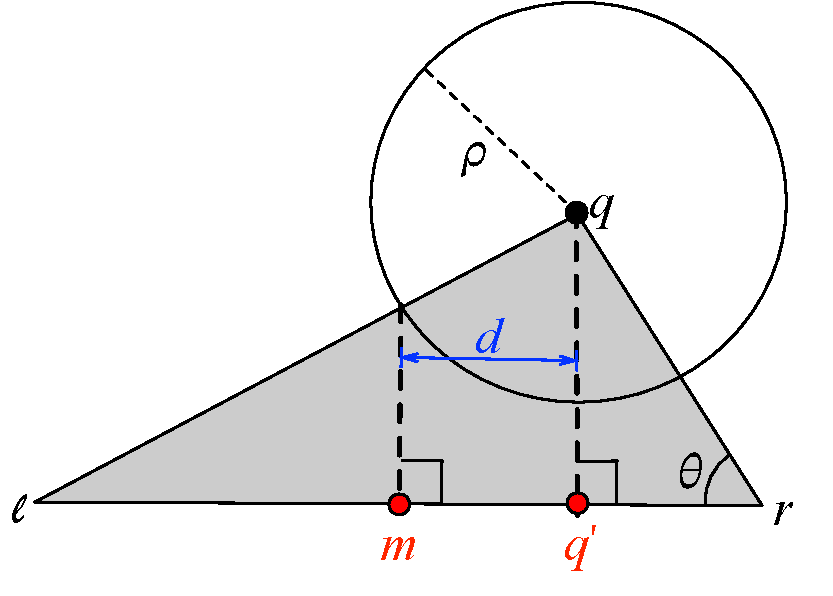
\includegraphics[scale=0.8]{images/geometry/overlapping-children-3.pdf}
    \caption{The geometry of a query ball overlapping with a cluster and either one or both of its children.}
    \label{fig:methods:overlapping-children}
\end{figure}

To determine whether both children can contain points in the query ball, we consider Figure~\ref{fig:methods:overlapping-children}.
Here, we overload the notation for $\overline{x y}$ to refer both to the line segment joining points $x$ and $y$ as well as to the length of that line segment.

Let $q$ denote the query, $\rho$ denote the search radius, and $l$ and $r$ denote the cluster's left and right poles respectively (see Section~\ref{sec:methods:clustering:building-the-tree}).
Without loss of generality, we assume that $\overline{q r \vphantom{l}} \leq \overline{q l}$.
Now let $q'$ be the projection of $q$ onto $\overline{l r}$, $m$ be the midpoint of $\overline{l r}$, and $d$ be the distance from $q'$ to $m$.
As a consequence of how we assign a point in the parent cluster to the left child in Algorithm~\ref{alg:methods:partition}, if $\rho < d$, then the left child cannot contain points inside the query ball.
In such a case we proceed to search only the right child.
Otherwise, we proceed with both children.

To check whether $d \leq \rho$, we note that

\begin{equation*}
    d = \overline{m q' \vphantom{l}} = \overline{m r \vphantom{l}} - \overline{q' r \vphantom{l}} = \frac{\overline{l r}}{2} - \overline{q' r \vphantom{l}}.
\end{equation*}

Let $\theta$ denote $\angle l r q$, as shown in Figure~\ref{fig:methods:overlapping-children}.
By the Law of Cosines on $\triangle l r q$, we have that

\begin{equation*}
    \text{cos}(\theta) = \tfrac{\overline{l r}^2 + \ \overline{q r \vphantom{l}}^2 - \ \overline{q l}^2}{2 \cdot \overline{l r} \cdot \overline{q r \vphantom{l}}}.
\end{equation*}

Since $\triangle r q q'$ is a right triangle, we also have that

\begin{equation*}
    \text{cos}(\theta) = \tfrac{\overline{q' r \vphantom{l}}}{\overline{q r \vphantom{l}}}.
\end{equation*}

Combining the previous two equations and solving for $\overline{q' r \vphantom{l}}$, we have that

\begin{equation*}
    \overline{q' r \vphantom{l}} = \tfrac{\overline{q r \vphantom{l}}^2 + \ \overline{l r}^2 - \ \overline{q l}^2}{2 \cdot \overline{l r}}.
\end{equation*}

Substituting for $\overline{q' r \vphantom{l}}$ in the equation for $d$, we have that

\begin{equation*}
    d = \tfrac{\overline{l r}}{2} - \tfrac{\overline{q r \vphantom{l}}^2 + \ \overline{l r}^2 - \ \overline{q l}^2}{2 \cdot \overline{l r}} = \tfrac{\overline{q l}^2 - \overline{q r \vphantom{l}}^2}{2 \cdot \overline{l r}}.
\end{equation*}

Thus,

\begin{equation}
    d \leq \rho \iff (\overline{q l} + \overline{q r \vphantom{l}})(\overline{q l} - \overline{q r \vphantom{l}}) \leq 2 \cdot \overline{l r} \cdot \rho.
    \label{eq:methods:overlapping-children}
\end{equation}

Note, in particular, that Equation~\ref{eq:methods:overlapping-children} only requires distances between real points, and so it can be used with any distance function, even when $q'$ and $m$ are not real points or cannot be imputed from the data.

To perform $\rho$-NN search, we first perform a coarse \textit{tree-search}, as outlined in Algorithm~\ref{alg:methods:rnn-search:tree-search}, to find the leaf clusters which overlap with the query ball or any clusters which lie entirely within the query ball.
Then, for all such clusters, we perform a finer-grained \textit{leaf-search}, as outlined in Algorithm~\ref{alg:methods:rnn-search:leaf-search}, to find all points which are no more than a distance $\rho$ from the query.

\begin{algorithm} 
    \caption{tree-search($C$, $q$, $\rho$)} 
    \label{alg:methods:rnn-search:tree-search} 
    \begin{algorithmic}[0]
        \Require $C$, a cluster
        \Require $q$, a query
        \Require $\rho$, a search radius

        \If{$C$ is a leaf \textbf{or} $\delta^+_C \leq \rho$}
            \State \textbf{return} $\{C\}$
        \Else

            \State $[l, r]$ $\Leftarrow$ \textit{pole}s of $C$
            \State $[L, R]$ $\Leftarrow$ \textit{children} of $C$

            \If{$\overline{q l} < \overline{q r \vphantom{l}}$}
                \State $[r, l] \Leftarrow [l, r]$
                \State $[R, L] \Leftarrow [L, R]$
            \EndIf

            \If{$(\overline{q l} + \overline{q r \vphantom{l}})(\overline{q l} - \overline{q r \vphantom{l}}) \leq 2 \cdot \overline{l r} \cdot \rho$}
                \State \textbf{return} tree-search($L, q, \rho$) $\cup$ tree-search($R, q, \rho$)
            \Else
                \State \textbf{return} tree-search($R, q, \rho$)
            \EndIf
        \EndIf
    \end{algorithmic}
\end{algorithm}

\begin{algorithm} 
    \caption{leaf-search($S$, $q$, $\rho$)} 
    \label{alg:methods:rnn-search:leaf-search} 
    \begin{algorithmic}[0]
        \Require $S$, a set of clusters
        \Require $q$, a query
        \Require $\rho$, a search radius

        \State $H \Leftarrow \emptyset$, a set of hits

        \For{$C \in S$}
            \If{$\delta^+_C \leq \rho$}
                \State $H$ $\Leftarrow$ $H \cup \{C\}$
            \Else
                \For{$p \in C$}
                    \If{$f(p, q) \leq \rho$}
                        \State $H$ $\Leftarrow$ $H \cup \{p\}$
                    \EndIf
                \EndFor
            \EndIf
        \EndFor

        \State \textbf{return} $H$
    \end{algorithmic}
\end{algorithm}

\begin{algorithm} 
    \caption{$\rho$-NN-search($root$, $q$, $\rho$)} 
    \label{alg:methods:rnn-search} 
    \begin{algorithmic}
        \Require $root$, the root cluster
        \Require $q$, a query
        \Require $\rho$, a search radius

        \State $S$ $\Leftarrow$ tree-search($root$, $q$, $\rho$)
        \State $H$ $\Leftarrow$ leaf-search($S$, $q$, $\rho$)
        \State \textbf{return} $H$
    \end{algorithmic}
\end{algorithm}

The asymptotic complexity of $\rho$-NN is the same as in~\cite{ishaq2019clustered} and shown in Equation~\ref{eq:methods:rnn-search-complexity}.

\begin{gather}
    \mathcal{O}
    \Bigg(
        \underbrace{
            \log~\overbrace{\mathcal{N}_{\hat{r}}(X)}^{\textrm{metric entropy}}
        }_{\textrm{tree-search}}
        \ + \ 
        \underbrace{
            \overbrace{ \big| B_X(q, \rho) \big|}^{\textrm{output size}}
            \overbrace{ \left( \frac{\rho + 2 \cdot \hat{r}}{ \rho} \right) ^ d}^{\textrm{scaling factor}}
        }_{\textrm{leaf-search}}
    \Bigg)
    \label{eq:methods:rnn-search-complexity}
\end{gather}
where $\hat{r}$ is the \textit{mean} radius of leaf clusters, $\mathcal{N}_{\hat{r}}(X)$ is the metric entropy at that radius, $B_X(q, \rho)$ is a ball of radius $\rho$ around the query $q$, and $d$ is the LFD around the query at the length scale of $\rho$ and $\rho + 2 \cdot \hat{r}$.

From Algorithm~\ref{alg:methods:rnn-search}, we have that $H = B_X(q, \rho)$, and so $\rho$-NN search performance scales linearly with the size of the output set and exponentially with the LFD around the query.
While one might worry that the exponential scaling factor would dominate, the manifold hypothesis suggests that the LFD of real-life datasets is typically very low, and so this algorithm actually scales sub-linearly with the cardinality of the dataset.


\subsection{\texorpdfstring{$k$}{k}-Nearest Neighbors Search}
\label{sec:methods:knn-search}

In this section, we present three novel algorithms for exact $k$-NN search:
Repeated $\rho$-NN, Breadth-First Sieve, and Depth-First Sieve.

In these algorithms, we use $H$, for \textit{hits}, to refer to the data structure which stores the closest points to the query found so far, and $Q$ to refer to the data structure which stores the clusters and points which are still in contention for being one of the $k$ nearest neighbors.


\subsubsection{Repeated \texorpdfstring{$\rho$}{p}-NN}
\label{sec:methods:knn-search:repeated-rnn}

In this algorithm, we perform $\rho$-NN search starting with a small search radius, and repeatedly increasing the radius until $|H| \geq k$.

Let the search radius $r$ be equal to the radius of the root cluster divided by the cardinality of the dataset.
We perform tree-search with radius $r$.
If no clusters are found, then we double $r$ and perform tree-search again, repeating until we find at least one cluster.
Let $Q$ be the set of clusters returned by the first tree-search which returns at least one cluster.

Now, so long as $\sum_{C \in Q} |C| < k$, we continue to perform tree-search, but instead of doubling $r$ on each iteration, we multiply it by a factor determined by the LFD in the vicinity of the query ball. 
In particular, we increase the radius by a factor of

\begin{equation}
    \min \left(2, \left( {\frac{k}{\sum_{C \in Q} |C|}} \right)^{\mu^{-1}} \right)
    \label{eq:methods:repeated-rnn-factor}
\end{equation}

where $\mu$ is the harmonic mean of the LFD of the clusters in $Q$.
We use the harmonic mean to ensure that $\mu$ is not dominated by outlier clusters with very high LFD.
We cap the radial increase at 2 to ensure that we do not increase the radius too quickly in any single iteration.

Intuitively, the factor by which we increase the radius should be \textit{inversely} related to the number of points found so far. 
When the LFD at the radius scale from the previous iteration is high, this suggests that the data are densely populated in that region.
Thus, a small increase in the radius would likely encounter many more points, so a smaller radial increase would suffice to find $k$ neighbors.
Conversely, when the LFD at the radius scale from the previous iteration is low, this suggests that the data are sparsely populated in that region.
In such a region, a small increase in the radius would likely encounter vacant space, so a larger radial increase is needed.
Thus, the factor of radius increase should also be \textit{inversely} related to the LFD.

Once $\sum_{C \in Q} |C| \geq k$, we are guaranteed to have found at least $k$ neighbors, and so we can stop increasing the radius.
We perform $\rho$-NN search with this radius and return the $k$ nearest neighbors.

\begin{algorithm} % enter the algorithm environment
    \caption{Repeated $\rho$-NN($root$, $q$, $k$)} % give the algorithm a caption
    \label{alg:methods:repeated-rnn} % and a label for \ref{} commands later in the document
    \begin{algorithmic}[0] % enter the algorithmic environment
        \Require $root$, the root cluster
        \Require $q$, a query
        \Require $k$, the number of neighbors to find

        \State $r \Leftarrow radius$ of the $root$ cluster
        \State $r \Leftarrow$ $\frac{r}{|root|}$

        \Loop
            \State $Q \Leftarrow$ tree-search($root$, $q$, $r$)
            \If{$Q \neq \emptyset$}
                \State \textbf{break}
            \EndIf
            \State $r \Leftarrow 2 \cdot r$
        \EndLoop

        \Loop
            \If{$\sum_{C \in Q} |C| >= k$}
                \State \textbf{break}
            \EndIf
            \State $\mu \Leftarrow \frac{|S|}{\sum_{C \in Q} \frac{1}{LFD(C)}}$
            \State $r \Leftarrow r \cdot \min \left( 2, \left( {\frac{k}{\sum_{C \in Q} |C|}} \right)^{\mu^{-1}} \right)$
            \State $S \Leftarrow$ tree-search($root$, $q$, $r$)
        \EndLoop

        \State $H \Leftarrow$ sort($\rho$-NN-search($root$, $q$, $r$))
        \State \textbf{return} $H[.. k]$
    \end{algorithmic}
\end{algorithm}


\subsubsection{Complexity of Repeated \texorpdfstring{$\rho$}{p}-NN}
\label{sec:methods:knn-search:repeated-rnn-complexity}

The complexity bounds for Repeated $\rho$-NN rely on the assumption that the query point is sampled from the same distribution as the rest of the data or, in other words, that it arises from the same generative process as the rest of the dataset.
Given the uses of $k$-NN search in practice, this assumption is reasonable.
From this assumption, we can infer that the LFD near the query does not differ significantly from the (harmonic) mean of the LFDs of clusters near the query at the scale of the distance from the query to the $k^{th}$ nearest neighbor.

We find it useful to adopt the terminology used in \cite{ishaq2019clustered} and \cite{yu2015entropy}, and address \textit{tree-search} and \textit{leaf-search} separately.
Tree-search refers to the process of identifying clusters which have overlap with the query ball, or in other words, clusters which might contain one of the $k$ nearest neighbors. 
Leaf-search refers to the process of identifying the $k$ nearest neighbors among the points in the clusters identified by tree-search.

In ~\cite{ishaq2019clustered}, we showed that the complexity of tree-search is $\mathcal{O}(\log\mathcal{N}_{\hat{r}}(X))$, where $\mathcal{N}_{\hat{r}}(X)$ is the metric entropy of the dataset $X$ at a radius $\hat{r}$.
To adjust this bound for Repeated $\rho$-NN, we must estimate the number of iterations of tree-search (Algorithm~\ref{alg:methods:rnn-search:tree-search}) needed to find a radius that guarantees at least $k$ neighbors.

Based on the assumption that the LFD near the query does not differ significantly from that of nearby clusters, Equation~\ref{eq:methods:repeated-rnn-factor} suggests that in the expected case, we need only two iterations of tree-search to find $k$ neighbors:
one iteration to find at least one cluster, and the one more to find enough the $k$ neighbors.
Since this is a constant factor, complexity of tree-search for Repeated $\rho$-NN is the same as that of $\rho$-NN search, i.e. $\mathcal{O}\big(\log\mathcal{N}_{\hat{r}}(X)\big)$.

To determine the asymptotic complexity of leaf-search, we must estimate $\sum_{C \in Q} |C|$, the total cardinality of the clusters returned by tree-search.
Since we must examine every point in each such clusters, time complexity of leaf-search is linear in $\sum_{C \in Q} |C|$. 
Let $\rho_k$ be the distance from the query to the $k^{th}$ nearest neighbor.
Then, we see that $Q$ is expected to be the set of clusters which overlap with a ball of radius $\rho_k$ around the query.
We can estimate this region as a ball of radius $\rho_k + 2\hat{r}$, where $\hat{r}$ is the mean radius of the clusters in $Q$.

The work in~\cite{yu2015entropy} showed that

\begin{equation*}
    \sum_{C \in S} |C| \leq \gamma  \left| B(q, \rho_k) \right| \left(\frac{\rho_k + 2 \cdot \hat{r}}{\rho_k} \right)^d
\end{equation*}

where $\gamma$ is a constant. 
By definition of $\rho_k$, we have that $|B(q, \rho_k)| = k$.
Thus,

\begin{equation*}
    \sum_{C \in S} |C| \leq \gamma k \left( 1 + 2 \cdot \frac{\hat{r}}{\rho_k} \right)^d
\end{equation*}

An estimate for $\rho_k$ is still needed. 
For this, we once again rely on the assumption that the query is drawn from the same distribution as the rest of the data, and thus the LFD at the query point is not significantly different from the LFD of nearby clusters.

We let $\hat{d}$ be the (harmonic) mean LFD of the clusters in $Q$.
While ordinarily we compute LFD by comparing cardinalities of two balls with two different radii centered at \textit{the same} point, in order to estimate $\rho_k$, we instead compare the cardinality of a ball \textit{around the query} of radius $\rho_k$ to the mean cardinality, $\hat{|C|}$, of clusters in $Q$ at a radius equal to the mean of their radii, $\hat{r}$.
We justify this approach by noting that, since the query is from the same distribution as the rest of the data, we could move from the query to the center of one of the nearby clusters without significantly changing our estimate of the LFD.

By Equation~\ref{eq:methods:lfd-original},

\begin{equation*}
    \hat{d} = \frac{\log{}\frac{\hat{|C|}}{k}}{\log{}\frac{\hat{r}}{\rho_k}}
\end{equation*}

We can rearrange this equation to get

\begin{equation*}
    \frac{\hat{r}}{\rho_k} = \left( \frac{\hat{|C|}}{k} \right)^{\hat{d}^{-1}}
\end{equation*}

Using this to simplify the term for leaf-search in Equation~\ref{eq:methods:rnn-search-complexity}, we get

\begin{equation*}
    k \left( 1 + 2 \cdot \left( \frac{\hat{|C|}}{k} \right) ^ {\hat{d}^{-1}} \right)^d.
\end{equation*}

In addition, by our assumption that the LFD at the query is not significantly different from the LFD of nearby clusters, we have that $\hat{d} \approx d$.
By combining the bounds for tree-search and leaf-search, we see that Repeated $\rho$-NN has an asymptotic complexity of

\begin{gather}
    \mathcal{O}
    \Bigg(
        \underbrace{
            \log~\overbrace{\mathcal{N}_{\hat{r}}(X)}^{\textrm{metric entropy}}
        }_{\textrm{tree-search}}
        \ + \ 
        \underbrace{
            \overbrace{k}^{\textrm{output size}}
            \overbrace{\bigg( 1 + 2 \cdot \Big( \frac{\hat{|C|}}{k} \Big) ^ {d^{-1}} \bigg)^d}^{\textrm{scaling factor}}
        }_{\textrm{leaf-search}}
    \Bigg)
    \label{eq:methods:repeated-rnn-complexity}
\end{gather}

where $\mathcal{N}_{\hat{r}}(X)$ is the metric entropy of the dataset, $d$ is the LFD of the dataset, and $k$ is the number of nearest neighbors.
We note that the scaling factor should be close to 1 unless fractal dimension is highly variable in the region around the query (i.e. if $\hat{d}$ differs significantly from $d$).


\subsubsection{Breadth-First Sieve}
\label{sec:methods:knn-search:bredth-first-sieve}

This algorithm performs a breadth-first traversal of the tree, pruning clusters by using a modified version of the QuickSelect algorithm~\cite{hoare1961algorithm} at each level.

We begin by letting $Q$ be a set of 3-tuples $(p, \delta^{+}_{p}, m)$, where $p$ is either a cluster or a point, $\delta^{+}_{p}$ is the $\delta^{+}$ of $p$ as illustrated in Figure~\ref{fig:methods:deltas}, and $m$ is the multiplicity of $p$ in $Q$.
During the breadth-first traversal, for every cluster $C$ we encounter, we add $(C, \delta^{+}_{C}, |C| - 1)$ and $(c, \delta_{c}, 1)$ to $Q$, where $c$ is the center of $C$.
Recall that by the definitions of $\delta$ and $\delta^{+}$ given in Section~\ref{sec:methods:the-search-problem}, since $c$ is a point, $\delta_{C} = \delta_{c} = \delta^{+}_{c} = \delta^{-}_{c}$.

We then use the QuickSelect algorithm, modified to account for multiplicities and to reorder $Q$ in-place, to find the element in $Q$ with the $k^{th}$ smallest $\delta^{+}$; in other words, we find $\tau$, the smallest $\delta^{+}$ in $Q$ such that $\left| B_X(q, \tau) \right| \geq k$.
Since this step may require a binary search for the correct pivot element to find $\tau$ and reordering with a new pivot takes linear time in the size of the input list, this version of QuickSelect has $\mathcal{O}(|Q| \log |Q|)$ time complexity.

We then remove from $Q$ any element for which $\delta^{-} > \tau$ because such elements cannot contain (or be) one of the $k$ nearest neighbors.
Next, we remove all leaf clusters from $Q$ and add their points to $Q$ instead.
Finally, we replace all remaining clusters in $Q$ with the pairs of 3-tuples corresponding to their child clusters.

We continue this process until $Q$ no longer contains any clusters.
We then use the QuickSelect algorithm one last time to reorder $Q$, find $\tau$, and return the $k$ nearest neighbors.

This process is described in Algorithm~\ref{alg:methods:bredth-first-sieve}. 

\begin{algorithm} % enter the algorithm environment
    \caption{Breadth-First Sieve($root$, $q$, $k$)} % give the algorithm a caption
    \label{alg:methods:bredth-first-sieve} % and a label for \ref{} commands later in the document
    \begin{algorithmic}[0] % enter the algorithmic environment
        \Require $root$, the root cluster
        \Require $q$, a query
        \Require $k$, the number of neighbors to find

        \State $c \Leftarrow$ \textit{center} of $root$
        \State $Q \Leftarrow$ \{ ($root$, $\delta^{+}_{root}$, $|root| - 1$), ($c$, $\delta_{root}$, 1) \}

        \Loop
            \If{$k = \sum_{(\_, \_, m) \in Q} m$}
                \State \textbf{break}
            \EndIf
            \State $\tau \Leftarrow$ QuickSelect($Q$, $k$)
            \For{$(p, \delta^{+}_{p}, m) \in Q$}
                \If{$\delta^{-}_{p} > \tau$}
                    \State $Q \Leftarrow Q \setminus \{ (p, \delta^{+}_{p}, m) \}$
                \EndIf
            \EndFor
            \For{$(p, \delta^{+}_{p}, m) \in Q$}
                \State $Q \Leftarrow Q \setminus \{ (p, \delta^{+}_{p}, m) \}$
                \If{$p$ is a point}
                    \State \textbf{continue}
                \ElsIf{$p$ is a leaf}
                    \For{$c \in p$}
                        \State $Q \Leftarrow Q \cup \{ (c, \delta_{c}, 1) \}$
                    \EndFor
                \Else
                    \State $[L, R] \Leftarrow$ children of $p$
                    \State $Q \Leftarrow Q \cup \{ (L, \delta^{+}_{L}, |L| - 1), (L_c, \delta_{L}, 1) \}$
                    \State $Q \Leftarrow Q \cup \{ (R, \delta^{+}_{R}, |R| - 1), (R_c, \delta_{R}, 1) \}$
                \EndIf
            \EndFor
        \EndLoop

        \State \textbf{return} $Q$
    \end{algorithmic}
\end{algorithm}


\subsubsection{Depth-First Sieve}
\label{sec:methods:knn-search:depth-first-sieve}

This algorithm performs a depth-first traversal of the tree and uses two priority queues to track clusters and hits.

Let $Q$ be a min-queue of clusters prioritized by $\delta^{-}$ and $H$ be a max-queue (with capacity $k$) of points prioritized by $\delta$.
$Q$ starts containing only the root cluster while $H$ starts empty.
So long as $H$ is not full or the top priority element in $H$ has $\delta$ greater than or equal to the top priority element in $Q$, we take the following steps:

\begin{itemize}
    \item While the top priority element $Q$ is not a leaf, remove it from $Q$ and add its children to $Q$.
    \item Remove the top priority element (a leaf) from $Q$ and add all its points to $H$.
    \item If $H$ has more than $k$ points, remove points from $H$ until $|H| = k$.
\end{itemize}

This process is described in Algorithm~\ref{alg:methods:depth-first-sieve}.
It terminates when $H$ is full and the top priority element in $H$ has $\delta$ less than the top priority element in $Q$, i.e., the theoretically closest point left to be considered in $Q$ is farther from the query than the $k^{th}$ nearest neighbor in $H$.
This leaves $H$ containing exactly the $k$ nearest neighbors to the query.


\begin{algorithm} 
    \caption{Depth-First Sieve($root$, $q$, $k$)} 
    \label{alg:methods:depth-first-sieve} 
    \begin{algorithmic}[0]
        \Require $root$, the root cluster
        \Require $q$, a query
        \Require $k$, the number of neighbors to find

        \State{$Q \Leftarrow [root]$, a min-priority queue by $\delta^{-}$}
        \State{$H \Leftarrow []$, a max-priority queue by $\delta$}

        \While{$|H| < k$ \textbf{or} $H.peek.\delta \geq Q.peek.\delta^{-}$}
            \While{$\neg (Q.peek$ is a leaf)}
                \State{$C \Leftarrow Q.pop$, the closest cluster}
                \State{$[L, R] \Leftarrow$ children of $C$}
                \State{$Q.push(L)$}
                \State{$Q.push(R)$}
            \EndWhile
            \State{$leaf \Leftarrow Q.pop$}
            \For{$p \in leaf$}
                \State{$H.push(p)$}
            \EndFor
            \While{$|H| > k$}
                \State{$H.pop$}
            \EndWhile
        \EndWhile
        \State Return $H$
    \end{algorithmic}
\end{algorithm}

Note that this algorithm is not truly a depth-first traversal of the tree in the classical sense, because we use $Q$ to prioritize which branch of the tree we descend into.
Indeed, we expect this algorithm to often switch which branch of the tree is being explored at greater depth.


\subsubsection{Complexity of Sieve Methods}
\label{sec:methods:knn-search:complexity-of-sieve-methods}

Due to their similarity, we combine the complexity analyses of the two Sieve methods into one section.
For these methods we, once again, use the terminology of tree-search and leaf-search.
Tree-search navigates the cluster tree and adds clusters to $Q$.
Leaf-search exhaustively searches some of the clusters in $Q$ to find the $k$ nearest neighbors.

We start with the assumption that the LFD near the query does not differ significantly from that of nearby clusters, and we consider leaf clusters with cardinalities near $k$.
Let $d$ be the LFD in this region.
Then the number of leaf-clusters in $Q$ is bounded above by $2d$, e.g. we could have a cluster overlapping the query ball at each end of each of $d$ mutually-orthogonal axes.
In the worst-case scenario for tree-search, these leaf clusters would all come from different branches of the tree, and so tree-search looks at $2 \cdot d \cdot \log \mathcal{N}_{\hat{r}}(X)$ clusters.
Thus, the asymptotic complexity is

\begin{equation*}
    \mathcal{T} \coloneqq \mathcal{O} \big( d \cdot \log \mathcal{N}_{\hat{r}}(X) \big).
\end{equation*}

For leaf-search, the output size and scaling factor are the same as in Repeated $\rho$-NN, and so the asymptotic complexity is

\begin{equation*}
    \mathcal{L} \coloneqq \mathcal{O} \left( k \cdot \bigg( 1 + 2 \cdot \Big( \frac{\hat{|C|}}{k} \Big) ^ {d^{-1}} \bigg)^d \right).
\end{equation*}

The asymptotic complexity of Breadth-First Sieve is dominated by the QuickSelect algorithm to calculate $\tau$.
Since this method is log-linear in the length of $Q$, and $Q$ contains the clusters from tree-search and the points from leaf-search, we see that the asymptotic complexity is

\begin{equation}
    \mathcal{O} \Big( ( \mathcal{T} + \mathcal{L} ) \log ( \mathcal{T} + \mathcal{L} ) \Big).
    \label{eq:methods:breadth-first-sieve-complexity}
\end{equation}

For Depth-First Sieve, since we use two priority queues, the asymptotic complexity is dominated by the complexity of the priority queue operations.
Thus, the asymptotic complexity is

\begin{equation}
    \mathcal{O} \Big( \mathcal{T} \log \mathcal{T} + \mathcal{L} \log k \Big).
    \label{eq:methods:depth-first-sieve-complexity}
\end{equation}


\subsection{Auto-Tuning}
\label{sec:methods:auto-tuning}

We perform some na\"{i}ve auto-tuning to select the optimal $k$-NN algorithm to use with a given dataset.
We start by taking the center of every cluster at a low depth, (e.g. 10), in the cluster tree as a query.
This gives us a small, representative sample of the dataset.
Using these clusters' centers as queries, and a user-specified value of $k$, we record the time taken for $k$-NN search on the sample using each of the three algorithms described in Section~\ref{sec:methods:knn-search}.
We select the fastest algorithm over all the queries as the optimal algorithm for that dataset and value of $k$.
Note that even though we select the optimal algorithm based on use with some user-specified value of $k$, we still allow search with any value of $k$.


\subsection{Synthetic Data}
\label{sec:methods:synthetic-data}

Based on our asymptotic complexity analyses, we expect CAKES to perform well on datasets with low LFD, and for its performance to scale sub-linearly with the cardinality of the dataset.
To test this hypothesis, we use some datasets from the ANN-benchmarks suite~\cite{aumuller2020ann} and synthetically augment them to generate similar datasets with exponentially larger cardinalities.
We do the same with a large random dataset of uniformly distributed points in a hypercube.
We then compare the performance of CAKES to that of other algorithms on the original datasets and the synthetically augmented datasets.

To elaborate on the augmentation process, we start with an original dataset from the ANN-benchmarks suite.
Let $X$ be the dataset, $d$ be its dimensionality, $\epsilon$ be a user-specified noise level, and $m$ be a user-specified integer multiplier.
For each datum $x \in X$, we create $m - 1$ new data points within a distance $\epsilon \cdot ||x||$ of $x$ where $||x||$ is the Euclidean distance from $x$ to the origin.
We construct a random vector $r$ of $d$ dimensions in the hyper-sphere of radius $\epsilon$ centered at the origin.
We then add $r$ to $x$ to get a new point $x'$.
Since $||r|| \leq \epsilon$, we have that $||x - x'|| \leq \epsilon$ (i.e., $x'$ is within a distance $\epsilon$ of $x$).
This produces a new dataset $X'$ with $|X'| = m \cdot |X|$.

This augmentation process preserves the topological structure of the original dataset, but increases its cardinality by a factor of $m$, allowing us to isolate the effect of cardinality on search performance from that of other factors such as dimensionality, choice of metric, or the topological structure of the dataset.
